\section{PERFORMANCE AND APPLICATIONS}

\begin{figure}[h]
  \centering
 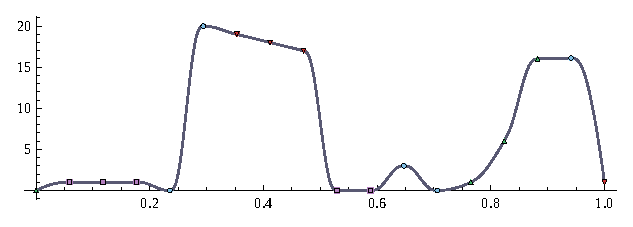
\includegraphics[width=4in]{vis/2-piecewise-polynomial.eps}
 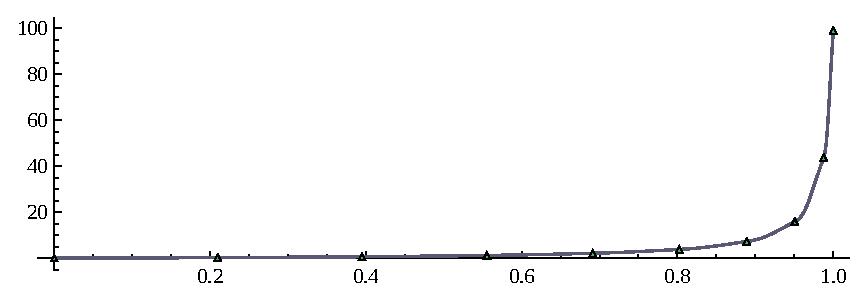
\includegraphics[width=4in]{vis/3-large-tangent.eps}
 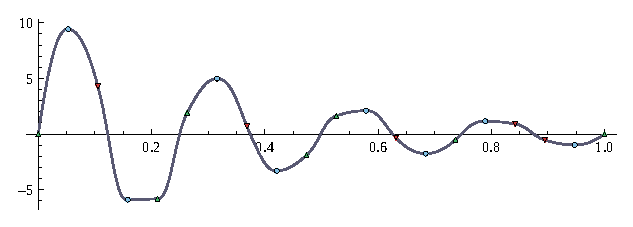
\includegraphics[width=4in]{vis/4-signal-decay.eps}
\caption{ % \narrower\noindent\rmVIII Fig.\ 2.
{\ttVIII MQSI} results for three of the functions in the included test
suite. The {\itVIII piecewise polynomial} function (top) shows the
interpolant capturing local linear segments, local flats, and
alternating extreme points. The {\itVIII large tangent} (middle)
problem demonstrates outcomes on rapidly changing segments of data.
The {\itVIII signal decay} (bottom) alternates between extreme values
of steadily decreasing magnitude.}
\end{figure}
  %% \vskip 6mm
\begin{figure}
  \centering
  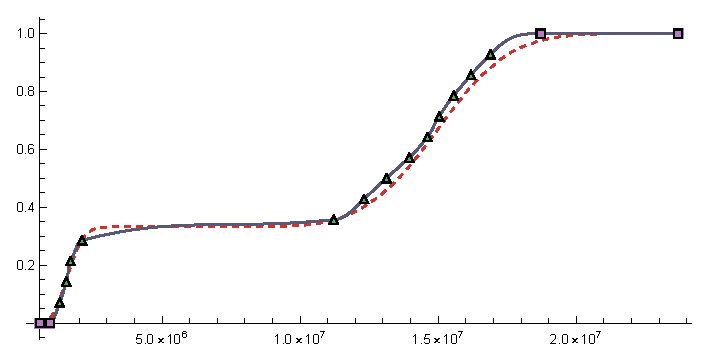
\includegraphics[width=4in]{vis/5-real-data.eps}
\caption{ % \narrower\noindent\rmVIII Fig.\ 3.
{\ttVIII MQSI} results when approximating the cumulative distribution
function of system throughput (bytes per second) data for a computer
with a 3.2 GHz CPU performing file read operations from Cameron et al.
\cite{cameron2019moana}. The empirical distribution of 30 thousand throughput values is
shown in the red dashed line, while the solid line with stylized
markers denotes the approximation made with {\ttVIII MQSI} given
equally spaced empirical distribution points from a sample of size 100.}
\end{figure}

\begin{figure}[h]
  \centering
  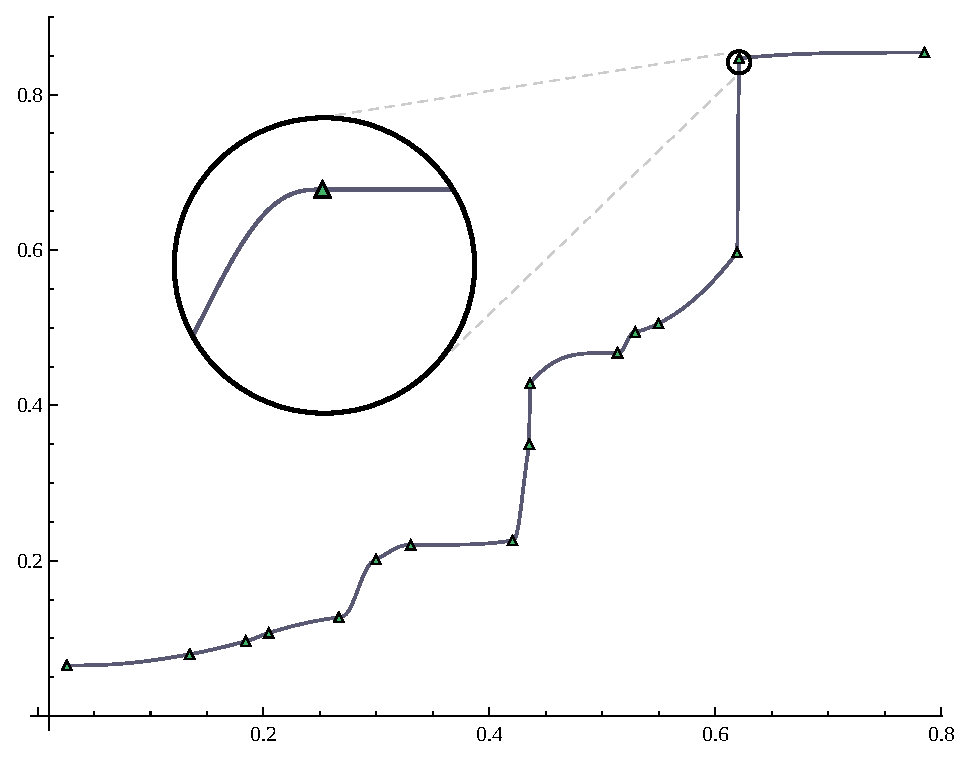
\includegraphics[width=4in]{vis/6-random-monotone.eps}
\caption{ % \narrower\noindent\rmVIII  Fig.\ 4.
The {\itVIII random monotone} test poses a particularly challenging
problem with large variations in slope. Notice that despite drastic
shifts in slope, the resulting monotone quintic spline interpolant
provides smooth and reasonable estimates to function values between data.}
\end{figure}

This section contains graphs of sample {\tt MQSI} results given various
data configurations. Execution times for Algorithms 1 and 4 are given; the
total execution time of {\tt MQSI} is utterly dominated by the time for a
banded linear system solve computing the $3n$ $B$-spline coefficients,
which is $\mathcal{O}(n)$.  The files {\tt sample\_main.f90} and {\tt
sample\_main.dat} accompanying the subroutine {\tt MQSI} illustrate Fortran
2003 subroutine usage with optional arguments and data points from a file.
Compilation instructions and the full package contents are specified in
the {\tt README} file.

Throughout, all visuals have points that are stylized by local
monotonicity conditions. Blue circles denote extreme points, purple
squares are in {\it flat} regions with no change in function value,
red down triangles are monotone decreasing, and green up triangles are
monotone increasing.

Figure 2 offers examples of the interpolating splines produced by the
routine {\tt MQSI} on various hand-crafted sets of data. These same
data sets are used for testing local installations in the provided
program {\tt test\_all.f90}. Notice that the quadratic facet model
perfectly captures the local linear segments of data in the piecewise
polynomial test for Figure 2. Figure 3 depicts an approximation of a
cumulative distribution function made by {\tt MQSI} on a computer
systems application by Cameron et al. \cite{cameron2019moana} that studies the
distribution of throughput (in bytes per second) when reading files
from a storage medium. Figure 4 provides a particularly difficult
monotone interpolation challenge using randomly generated monotone
data.

On a computer running MacOS 10.15.5 with a 2 GHz Intel Core i5 CPU, the
quadratic facet (Algorithm 1) takes roughly one microsecond ($10^{-6}$
seconds) per breakpoint, while the binary search (Algorithm 4) takes roughly
four microseconds per breakpoint; these times were generated from 100
repeated trials averaged over 14 different testing functions.  The vast
majority of execution time is spent solving the banded linear system of
equations in the routine {\tt FIT\_SPLINE} for the $B$-spline coefficients.
For large problems ($n > 100$) it would be faster to construct splines
over intervals independently (each interval requiring a $6 \times 6$ linear
system to be solved for a local $B$-spline representation, or the
construction of the Newton form of the interpolating polynomial from the
derivative information at the endpoints), however the single linear system
is chosen here for the decreased redundancy in the spline description. An
optional argument to {\tt MQSI} returns the derivative information at the
breakpoints (interval endpoints) for the Newton form of the interpolating
polynomial (piece of $Q(x)$) over each interval.

Lastly, comparisons between {\tt MQSI} and four published spline
software packages are provided that allow subjective inspection on the
same four test problems as presented above. In each of Figures 5
through 8 the intricacies of the approximation created by {\tt MQSI}
can be contrasted with two monotone $C^1$ quadratic splines (TOMS 574,
and Schumaker), the popular $C^1$ piecewise cubic method {\tt PCHIP},
and the $C^2$ piecewise quintic method {\tt BVSPIS} of TOMS
770. Figures 5 and 8 demonstrate glaring numerical errors in the
Schumaker and {\tt BVSPIS} implementations. Minimum working examples
that reproduce similar errors are provided in the associated software
{\tt test\_schumaker.r} and {\tt test\_bvspis.f03}. The failure modes
of these published codes are surprising, but also accentuate how
difficult it is to correctly handle the numerical complexities of
polynomial function evaluation.

Overall it can be observed that the minimal and tight conditions on
monotonicity provided by TOMS 574 tend to be more visually appealing
than the weaker sufficient conditions utilized by {\tt PCHIP}. In
general the major determining factor for the quality of {\tt MQSI} is
the local quadratic facet model. For applications where the underlying
function is presumed to be a piecewise polynomial (of relatively low
order), the choice of local quadratic interpolants is
reasonable. However the consequence of this decision is that functions
with superquadratic rates of change will tend to have consistently
underestimated first and second derivatives. This limitation is
accepted in favor of perfectly capturing lower order phenomena. Were
future research to supply alternative initializations for $C^2$
quintic splines, those could comfortably be made monotone by the
procedures of {\tt MQSI} and most importantly by the application of
these sharp monotonicity conditions.

If an application demands $C^2$ continuity and monotonicity, the
target of {\tt MQSI}, then this package uniquely provides such
interpolants based on sharp monotonicity constraints.

\goodbreak

\begin{figure}[h]
  \centering
\includegraphics[width=4in]{vis/comparisons/piecewise-polynomial/1-toms574.eps}
\includegraphics[width=4in]{vis/comparisons/piecewise-polynomial/2-schumaker.eps}
\includegraphics[width=4in]{vis/comparisons/piecewise-polynomial/3-pchip.eps}
\includegraphics[width=4in]{vis/comparisons/piecewise-polynomial/4-bvspis.eps}
\caption{ % \narrower\noindent\rmVIII Fig.\ 5.
{\ttVIII MQSI} compared with each of TOMS 574 (first, blue), Schumaker
(second, red), {\ttVIII PCHIP} (third, green), and {\ttVIII BVSPIS}
(fourth, purple) respectively on the {\itVIII piecewise polynomial}
test function. {\ttVIII MQSI} is styled as a gray thin line in the
background for comparison. The Schumaker code (second) fails to
produce a monotone approximation for this problem while producing no
errors or warnings. The primary comparative observation of {\ttVIII
  MQSI} otherwise is its exact reproduction of the linear segment
between $0.3$ and $0.5$.}
\end{figure}

\begin{figure}[h]
  \centering
\includegraphics[width=4in]{vis/comparisons/large-tangent/1-toms574.eps}
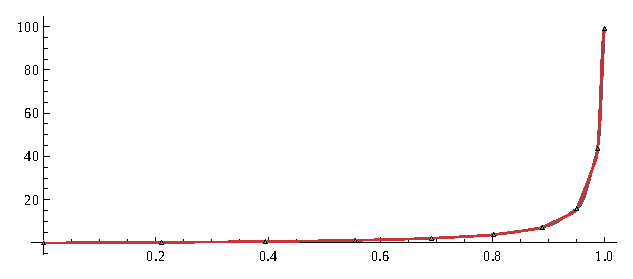
\includegraphics[width=4in]{vis/comparisons/large-tangent/2-schumaker.eps}
\includegraphics[width=4in]{vis/comparisons/large-tangent/3-pchip.eps}
\includegraphics[width=4in]{vis/comparisons/large-tangent/4-bvspis.eps}
\caption{ % \narrower\noindent\rmVIII Fig.\ 6.
{\ttVIII MQSI} compared with each of TOMS 574 (first, blue), Schumaker
(second, red), {\ttVIII PCHIP} (third, green), and {\ttVIII BVSPIS}
(fourth, purple) respectively on the {\itVIII large tangent} test
function. {\ttVIII MQSI} is styled as a gray thin line in the
background for comparison. This problem highlights the core weakness
of the quadratic facet model approach to derivative estimation in
{\ttVIII MQSI}, which consistently underestimates the actual
second derivative of this function. This weakness is accepted
for its greater accuracy when estimating local lower order components
of functions.}
\end{figure}

\begin{figure}
  \centering
\includegraphics[width=4in]{vis/comparisons/signal-decay/1-toms574.eps}
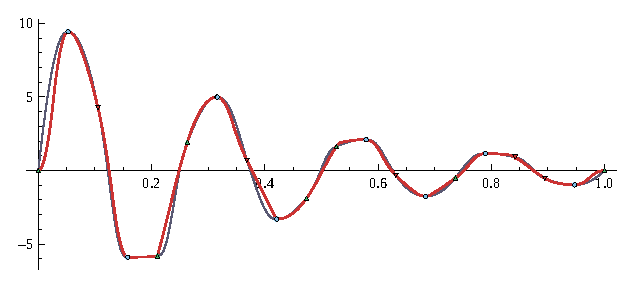
\includegraphics[width=4in]{vis/comparisons/signal-decay/2-schumaker.eps}
\includegraphics[width=4in]{vis/comparisons/signal-decay/3-pchip.eps}
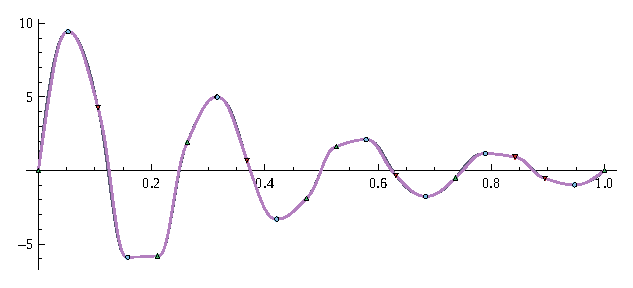
\includegraphics[width=4in]{vis/comparisons/signal-decay/4-bvspis.eps}
\caption{ % \narrower\noindent\rmVIII Fig.\ 7.
{\ttVIII MQSI} compared with each of TOMS 574 (first, blue), Schumaker
(second, red), {\ttVIII PCHIP} (third, green), and {\ttVIII BVSPIS}
(fourth, purple) respectively on the {\itVIII signal decay} test
function. {\ttVIII MQSI} is styled as a gray thin line in the
background for comparison. The most notable differences between
{\ttVIII MQSI} and other approaches can be observed near local
extrema, where {\ttVIII MQSI} produces continuous and smaller
magnitude second derivatives.}
\end{figure}

\begin{figure}
  \centering
\includegraphics[width=4in]{vis/comparisons/random-monotone/1-toms574.eps}
\includegraphics[width=4in]{vis/comparisons/random-monotone/2-schumaker.eps}
\includegraphics[width=4in]{vis/comparisons/random-monotone/3-pchip.eps}
\includegraphics[width=4in]{vis/comparisons/random-monotone/4-bvspis.eps}
\caption{ % \narrower\noindent\rmVIII Fig.\ 8.
{\ttVIII MQSI} compared with each of TOMS 574 (first, blue), Schumaker
(second, red), {\ttVIII PCHIP} (third, green), and {\ttVIII BVSPIS}
(fourth, purple) respectively on the {\itVIII random monotone} test
function. {\ttVIII MQSI} is styled as a gray thin line in the
background for comparison. Notice that the numerical conditions for
this approximation problem are challenging enough that both the
Schumaker and {\ttVIII BVSPIS} codes incorrectly produce nonmonotone
segments (neither of which produced error codes or any indication that
a failure occurred). Notably only {\ttVIII MQSI} and TOMS 574 satisfy
tight monotonicity constraints while also correctly preserving
monotonicity in their approximations, and only {\ttVIII MQSI} is
$C^2$. The main segment of divergence between the methods happens on
the $(0.45, 0.5)$ interval, where {\ttVIII MQSI} favors maximizing the
slope on the left side of the interval because the quadratic
interpolant of the right sided points produces a negative
slope estimate (invalid) on the left side of the interval.}
\end{figure}
